%!TEX root=../ctl-phd-thesis.tex

\section{Abstract}
\par Prediction of passive permeation rates of solutes across lipid bilayers is important to drug design, toxicology and other biological processes such as signaling. The inhomogeneous solubility-diffusion (ISD) equation is traditionally used to relate the position-dependent potential of mean force and diffusivity to the permeability coefficient. The ISD equation is derived via the Smoluchowski equation and assumes over-damped system dynamics. It has been suggested that the complex membrane environment may exhibit more complicated damping conditions. Here we derive a variant of the inhomogeneous solubility diffusion equation as a function of the mean first passage time (MFPT) and show how milestoning, a method that can estimate kinetic quantities of interest, can be used to estimate the MFPT of membrane crossing and, by extension, the permeability coefficient. We further describe a second scheme, agnostic to the damping condition, to estimate the permeability coefficient from milestoning results or other methods that compute a probability of membrane crossing. The derived relationships are tested using a 1-D Langevin dynamics toy system and confirmed that the presented theoretical methods can be used to estimate permeabilities given simulation and milestoning results.

\section{Introduction}
    \par Passive transport of solutes across membranes is of key importance for processes such as the uptake and excretion of drug compounds. Poor permeability can cause unfavorable pharmacokinetics or bioavailability leading to drug attrition\cite{Kola2004}. From this perspective of drug design, methods which provide molecular level insight into the permeation process are of high interest. As such, many physical models of permeability have been developed; these methods are recently reviewed\cite{Swift2013}.

    \par Mathematically, the permeability coefficient $P$ of a solute is described by relating the flux per unit area, $J$, across a bilayer and the concentration gradient, $\Delta u$, as
    \begin{equation}
        P = \frac{J}{\Delta u}.
        \label{eq:ficks1st}
    \end{equation}
    From this relation, assuming over-damped conditions and accounting for drift caused by the potential of mean force (PMF) we get the inhomogeneous solubility-diffusion equation (ISD)\cite{Marrink1994,Woolf1994,Bemporad2004,Xiang2006,Awoonor-Williams2015}:
    \begin{equation}
        P = \frac{1}{R} = \left[\int_{z_1}^{z_2}\frac{\exp(\beta W(z))}{D(z)}dz\right]^{-1},
        \label{eq:ihsd}
    \end{equation}
    where $R$ is the resistivity, $\beta = 1/k_BT$ where $T$ is the temperature, $k_B$ is Boltzmann's constant, $W(z)$ is the PMF, $D(z)$ is the local diffusivity constant and $z_1$, $z_2$ are two positions just outside of opposing sides of the membrane. Estimates of $W(z)$ and $D(z)$ can be predicted using molecular dynamics (MD) simulations\cite{Xiang2006,Swift2013,Awoonor-Williams2015}.     While the ISD has been applied successfully in many studies\cite{Wilson1996,Grossfield2002,Ulander2003a,Bemporad2004,MacCallum2007,Johansson2008,MacCallum2008,Bauer2011,Tejwani2011,MacCallum2011,Paloncyova2012,Swift2013,Riahi2014,Carpenter2014,Issack2015,Bemporad2005,Comer2014a}, recent work by various groups has suggested that the dynamics of crowded environments, such as inside the bilayer, may exhibit more complicated behaviors\cite{McGuffee2010,Swift2013}. The dynamics inside of the bilayer has not, to the best of our knowledge, been probed in detail\cite{Swift2013}.


    \par The theory of milestoning is a promising new approach to study molecular processes by employing many unbiased short independent simulations in subregions of phase space to predict thermodynamic and kinetic properties of interest. Salient descriptions of milestoning theory can be found in Refs.~\citenum{Faradjian2004,Majek2010,Kirmizialtin2011}. Previously, milestoning has been applied to the permeability problem by Cardenas et al., studying the permeation of block tryptophan across a membrane\cite{Cardenas2012}. Cardenas et al. later studied the permeation of small peptide NATA across a DOPC bilayer using milestoning. In their later work, they proposed a scheme to estimate the permeability coefficient\cite{Cardenas2013,Cardenas2014}. This scheme is comprised of three steps involving: 1) estimating the diffusivity of the small molecule in bulk, 2) the measurement of the steady state flux from bulk into the membrane, 3) estimation of permeant crossing probability. We will show that the additional calculations in step 2 are not necessary and the permeability can be computed directly from the milestoning results and bulk diffusivity.

    \par In this work we derive two methods for obtaining permeability coefficients based on milestoning results. The first derivation is a new formulation of the ISD relating the MFPT to the permeability coefficient $P$ assuming over-damped dynamics. The second derivation makes no assumptions about system damping, and relates $P$ to the transition probability of crossing a membrane over diffusing to a previous position in bulk solvent. We evaluate the compatibility of using either approach depending on damping dynamics using a 1-D Langevin dynamics system across various $W(z)$ and $D(z)$ profiles, showing that the new relations yield solutions in good accord with previous results.

\section{Theory}
    \subsection{Relating permeability to mean first passage time via the Smoluchowski equation}
        \begin{figure}[htbp]
        \begin{center}
            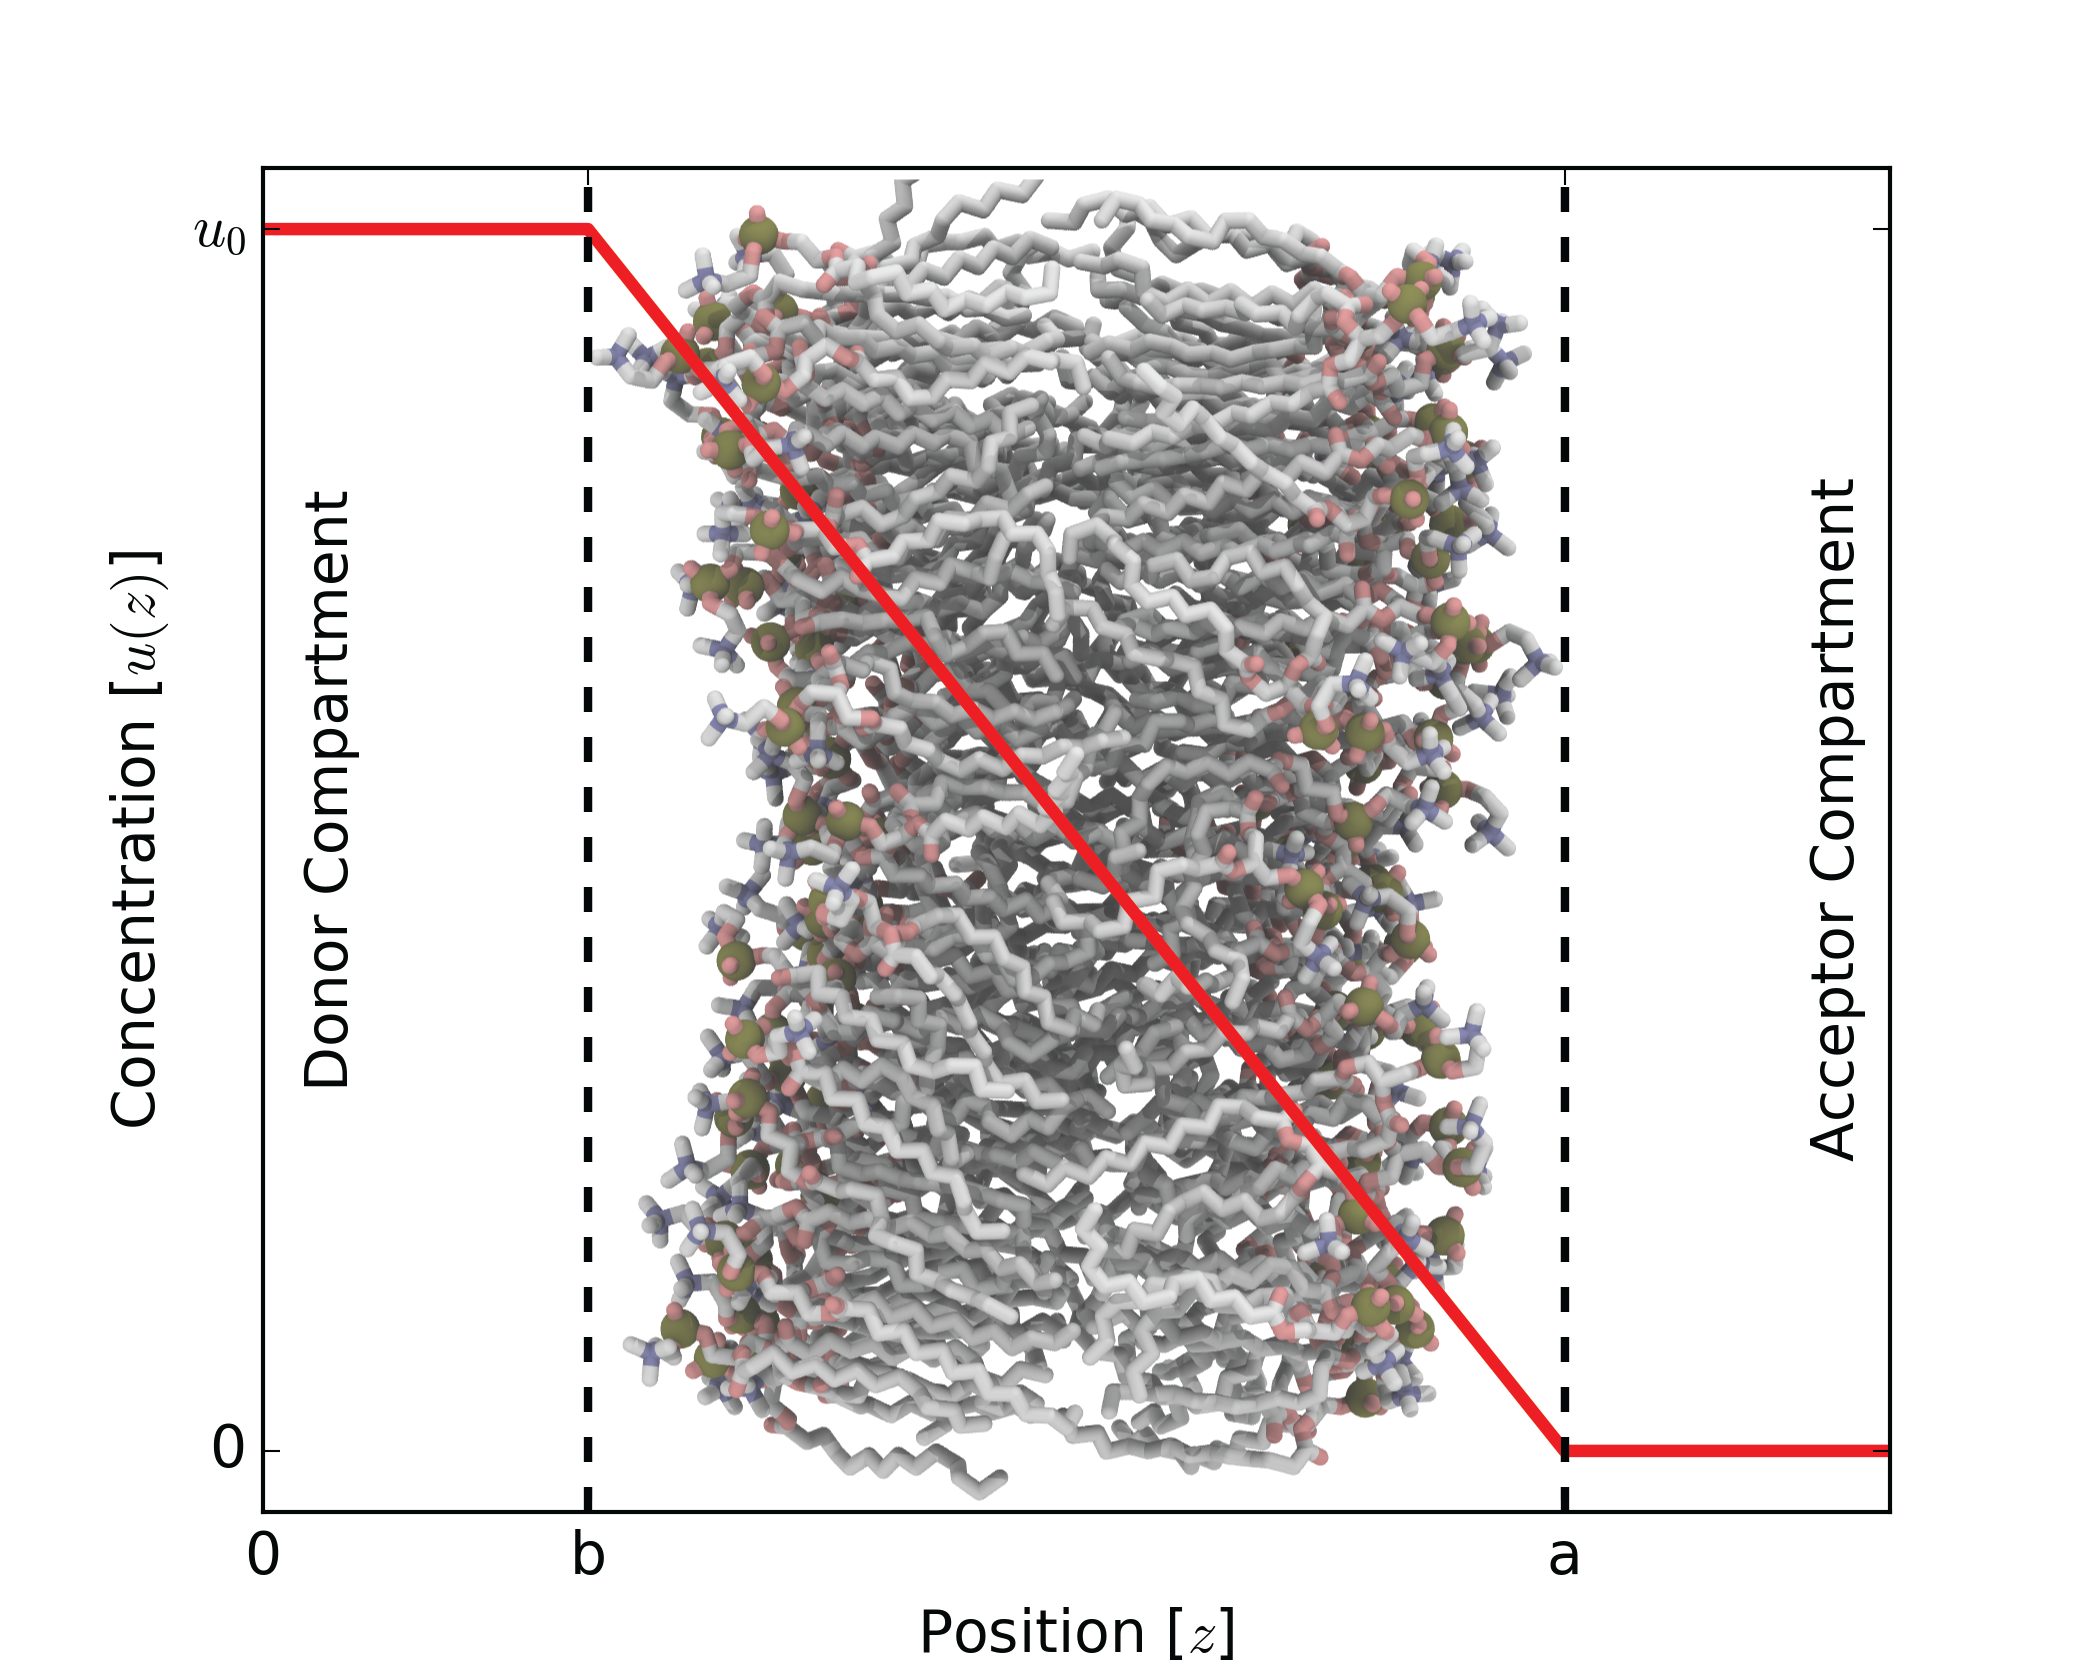
\includegraphics[width=0.8\textwidth]{Figures/ISD}
            \caption[Schematic of boundary conditions for the inhomogenous solubility-diffusion equation]{Schematic of membrane permeability showing the concentration of permeant with respect to position. We define that the concentration at $z=b$ is $u_0$ and $z=a$ is $0$. Assuming over-damped dynamics along with these boundary conditions, we get the inhomogeneous solubility-diffusion equation and its relation to passage time.}
            \label{fig:ISD}
        \end{center}
        \end{figure}

        \par The physical description of permeability can be drawn as a membrane separating donor and acceptor compartments (Fig.~\ref{fig:ISD}). Assuming that the dynamics are overdamped, permeation across a membrane can be modeled as a one-dimensional process using the 1-D Smoluchowski equation
        \begin{equation}
            \parfrac{u(z,t)}{t} = -\parfrac{J(z,t)}{z} = \frac{\partial}{\partial z}\left(D(z)\parfrac{u(z,t)}{z} - v(z,t)\cdot u(z,t)\right),
            \label{eq:smoluchowski}
        \end{equation}

        where $u(z,t)$ is the probability distribution at position $z$ and time $t$, $v(z,t)$ is the drift velocity, and $J(z,t)$ is the infinitesimal flux. A particle travels through a viscous medium at velocity $v = F(z)/\gamma$, where $F$ is the force on the particle and $\gamma$ is the friction coefficient. Using the Smoluchowski-Einstein relation $\gamma^{-1} = \beta D$, assuming steady-state conditions, and applying that $F = -\frac{dW(z)}{dz}$, we can convert the partial differential equation into an ordinary differential equation
        \begin{equation}
            0 = \frac{d}{dz} \left(D(z) \left[\frac{du(z)}{dz} + \frac{d \beta W(z)}{dz}u(z)\right]\right).
        \end{equation}
        Integrating and multiplying by $\frac{e^{\beta W(z)}}{D(z)}$, we get
        \begin{equation}
            e^{\beta W(z)} \frac{A_1}{D(z)} = \frac{du(z)}{dz} e^{\beta W(z)} + u(z)\frac{d\beta W(z)}{dz} e^{\beta W(z)},
            \label{eq:a1dz}
        \end{equation}
        where $A_1$ is a constant. The RHS can be condensed into a single differential
        \begin{equation}
            \frac{A_1}{D(z)} e^{\beta W(z)} = \frac{d}{dz}\left(u(z)e^{\beta W(z)}\right).
        \end{equation}
        By integrating, we can obtain a general expression for the steady-state concentration
        \begin{equation}
            u(z) = A_1e^{-\beta W(z)}\left(\int_0^z \frac{e^{\beta W(z')}}{D(z')}dz' \right) + A_2e^{-\beta W(z)}.
            \label{eq:uz}
        \end{equation}
        We now apply the boundary conditions shown in Fig.~\ref{fig:ISD}. Assuming that the acceptor compartment is a sink, $u(a) = 0$, and that in bulk $W(a) = 0$,
        \begin{equation}
            0 = A_1\left(\int_{0}^{a}\frac{e^{\beta W(z')}}{D(z')}dz'\right) + A_2.
        \end{equation}
        Solving for $A_2$
        \begin{equation}
            A_2 = -A_1\int_{0}^{a}\frac{e^{\beta W(z')}}{D(z')}dz'.
            \label{eq:a2}
        \end{equation}

        Substituting Eq.~\ref{eq:a2} into Eq.~\ref{eq:uz}, we get a difference of two integrals. Combining them into a single integral and setting the concentration of the donor compartment at position $b$ to that of bulk $u_0$
        \begin{equation}
            u(b) = u_0 = A_1e^{-\beta W(b)}\left(\int_a^b \frac{e^{\beta W(z')}}{D(z')}dz'\right).
        \end{equation}
        We can solve for the constant $A_1$
        \begin{equation}
            A_1 = \frac{u_0}{\int_a^b \frac{e^{\beta W(z')}}{D(z')}dz'} = -\frac{u_0}{\int_b^a \frac{e^{\beta W(z')}}{D(z')}dz'}.
            \label{eq:a1}
        \end{equation}
        Combining Eqs.~\ref{eq:a1}, \ref{eq:a2}, \ref{eq:uz}, the concentration $u(z)$ can be expressed according to
        \begin{equation}
            u(z) = \frac{-u_0 e^{-\beta W(z)}\left(\int_a^z\frac{e^{\beta W(z')}}{D(z')}dz'\right)}{\int_b^a \frac{e^{\beta W(z'')}}{D(z'')}dz''}.
            \label{eq:uzsolved}
        \end{equation}
        Returning to the calculation of the stationary flux, substituting Eq.~\ref{eq:a1dz} into Eq.~\ref{eq:smoluchowski}, and recognizing that the flux is just the negative of our first constant of integration, we get that
        \begin{equation}
            J = -A_1 = \frac{u_0}{\int_b^a\frac{e^{\beta W(z')}}{D(z')}dz'}.
        \end{equation}
        Substituting into Eq.~\ref{eq:ficks1st} and assuming that $\Delta u = u_0$, we get the ISD
        \begin{equation}
            P = \left[\int_b^a\frac{e^{\beta W(z')}}{D(z')}dz'\right]^{-1}
        \end{equation}

    \subsubsection{Mean First Passage Time}
        \par The MFPT $\mfptm$ of a diffusional encounter can be generally expressed as\cite{Hardt1981}
        \begin{equation}
            \mfptm = \frac{\int_v udV}{\sum_{i=1}^{m} \int_{A_i} J(A_i) dA_i},
        \end{equation}
        here $V$ is the total volume of the system in question, $m$ is the total number of isolated sinks, and $A_i$ is the total area of the $i$th sink. In our 1-D case, the expression is simplified:
        \begin{equation}
            \mfptm = \frac{\int_b^a u(z')dz'}{J(a)}.
        \end{equation}
        Taking the integral of Eq.~\ref{eq:uzsolved}, and reversing the order of integration in the numerator, we get
        \begin{equation}
            \int_b^a u(z)dz = \int_b^a\frac{u_0e^{-\beta W(z)} \left[\int_z^a \frac{e^{\beta W(z')}}{D(z')}dz'\right]}{\int_b^a \frac{e^{\beta W(z'')}}{D(z'')}dz''}dz.
        \end{equation}
        Noting the equivalence of $\int_b^a\int_z^a f(x)dx dz = \int_b^a\int_b^z f(x) dxdz$ for symmetrical functions over ${z|b<z<a}$ and dividing by $J(a) = -A_1$ we get
        \begin{equation}
            \mfptm = -\int_b^a e^{-\beta W(z)} \left[\int_b^z \frac{e^{\beta W(z')}}{D(z')}dz'\right]dz.
            \label{eq:mfpt}
        \end{equation}
        The MFPT can be related to the permeability coefficient by integrating Eq.~\ref{eq:mfpt} by parts
        \begin{equation}
            \mfptm = \left[\int_b^a e^{-\beta W(z)} dz\right] \left[\int_b^a\frac{e^{\beta W(z)}}{D(z)}dz\right] - \underbrace{\int_b^a \frac{e^{\beta W(z)}}{D(z)}\left[\int_b^z e^{-\beta W(z')}dz'\right]dz}_{\mfptm},
        \end{equation}
        where the second term on the RHS has been shown to be equal to the MFPT by others\cite{Schulten1981,Nadler1985,Ulander2003a,Cardenas2012} and can be derived by applying Fubini's theorem. Rewriting in terms of P and \mfpt
        \begin{equation}
            \mfptm = \frac{1}{P}\int_b^ae^{-\beta W(z)}dz - \mfptm
        \end{equation}
        and rearranging we get the permeability as it relates to \mfpt
        \begin{equation}
            P = \frac{\int_b^a e^{-\beta W(z)}dz}{2\mfptm}.
            \label{eq:permmfpt}
        \end{equation}
        This is formally equivalent to the ISD and obviates the calculation of the local diffusivity, requiring only the local PMF (or equivalently, the local stationary concentration of the permeant) and the MFPT.

    \subsection{Permeability from milestoning using crossing probability}
        \par Our second permeability derivation in this section is very similar to that used in Brownian dynamics (BD) simulations that make use of the Northrup-Allison-McCammon (NAM) algorithm\cite{Northrup1984}. As in BD simulations, the \surf{b} is the starting position of particles in the simulations. Conversely, the \surf{q} and \surf{a} are absorbing boundaries during the simulations. The quantity $\rho$ is the proportion of permeants that start at the \surf{b} and cross the membrane to touch the \surf{a} and not ``escape'' to the \surf{q}. Here, we attempt to be consistent with notation used in the NAM derivation. The only exception is that NAM uses a $\beta$ to represent the probability of crossing the \surf{a}, but we use the symbol $\rho$ instead to avoid confusion with the thermodynamic $\beta$ used in the previous section. This probability $\rho$ can be found using milestoning.

        \begin{figure}[htbp]
        \begin{center}
            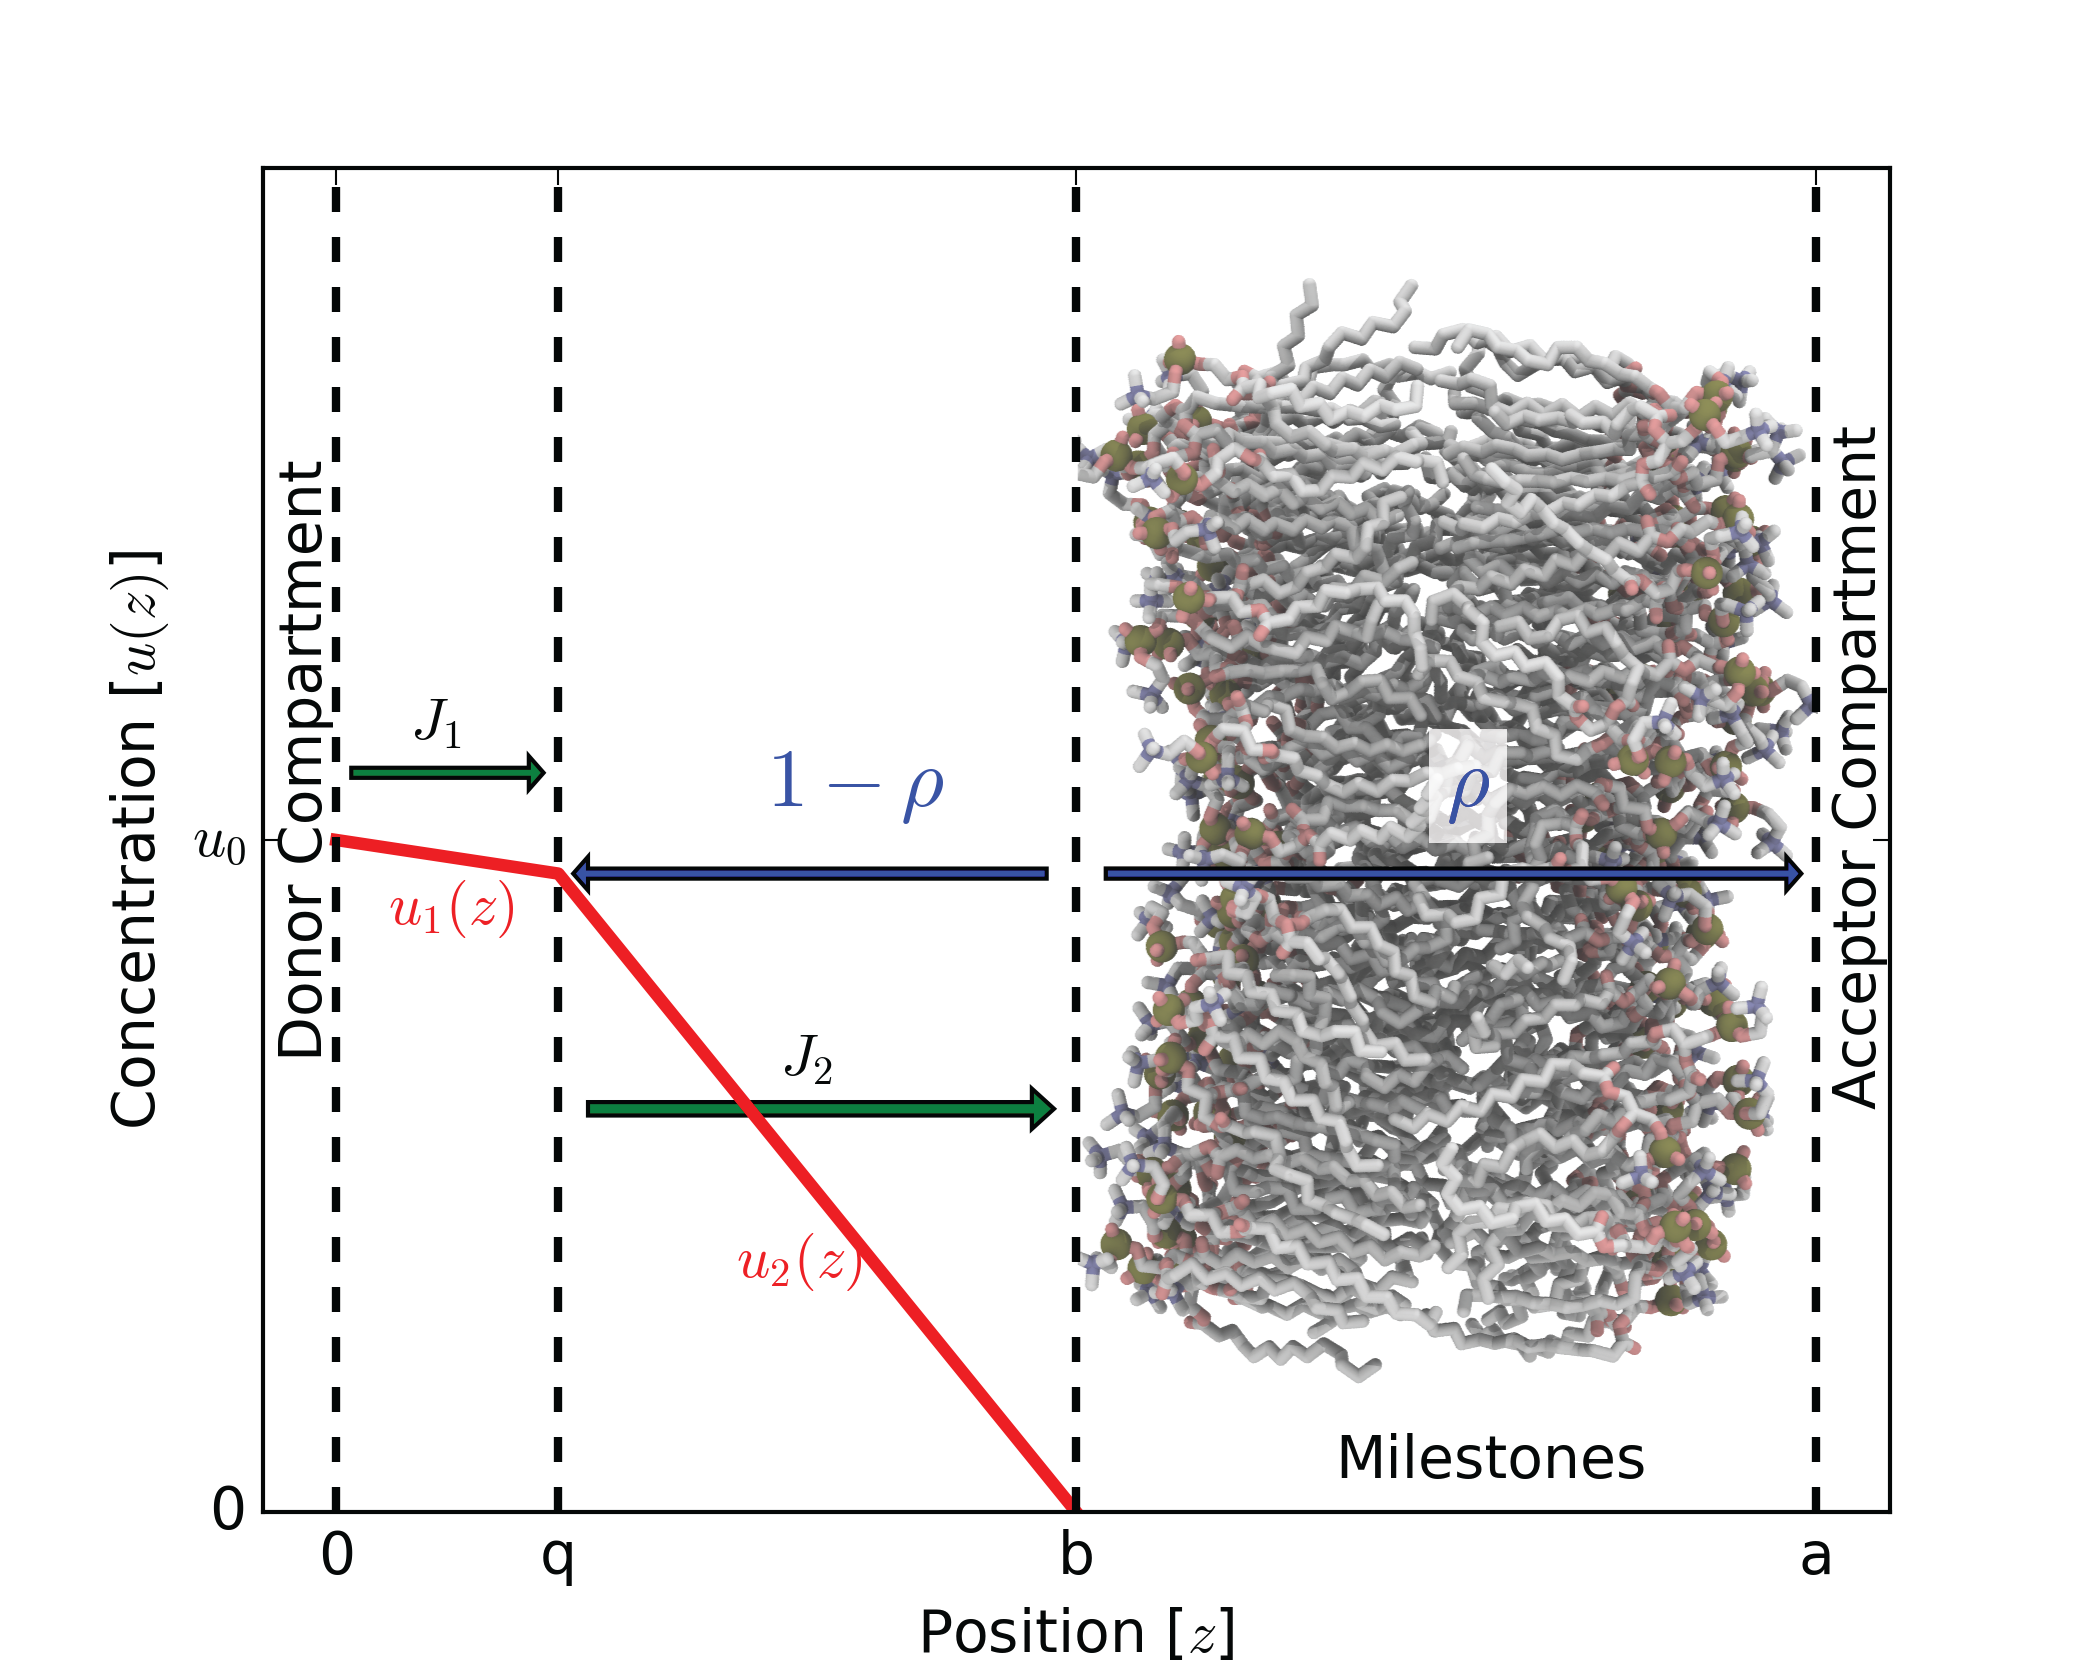
\includegraphics[width=0.8\textwidth]{Figures/probplot}
            \caption[Boundary conditions for computing permeability using milestoning]{Shown here is the milestoning system setup. The stationary concentrations in the bulk $u_1$ and $u_2$ are subject to boundary conditions at $z=0$ and $z=b$. A permeant that hits the \surf{b} has a probability of $\rho$ to cross the membrane and a probability $1-\rho$ to return to the \surf{q}. These boundaries and domains are not necessarily drawn to scale.}
            \label{fig:prob}
        \end{center}
        \end{figure}

        \par We define one additional surface in bulk solution on the donor side of the membrane: \surf{0} (placed at $z=0$ for mathematical convenience). Note that $a>b>q>0$. A steady-state Smoluchowski problem (Fig.~\ref{fig:prob}) is set up in the bulk domain between the \surf{0} and the \surf{b}, where the concentration at the \surf{0} boundary is held at $u_0$ and the concentration at the \surf{b} is held at $0$. Any flux across the \surf{b} has a probability equal to $\rho$ that it will be taken across the membrane and $1-\rho$ to return to the \surf{q}. Under this scheme, the permeability from the \surf{0} to \surf{a} can be found according to
        \begin{equation}
            P_{0\rightarrow a} = J(a)/u_0,
        \end{equation}
        where $u_0$ is the difference between the concentration at the \surf{0} and the concentration at the \surf{a}, and $J(a)$ is the flux across the \surf{a}. Since we assume steady-state conditions, the flux across the \surf{a} must be equal to the flux across the \surf{0}
        \begin{equation}
            P_{0\rightarrow a} = J(0)/u_0.
        \end{equation}

        \par Due to the fact that the region between the \surf{0} and \surf{b} exists in bulk solution, we assume that the PMF is constant and the dynamics over-damped, and we can use a 1-D Smoluchowski equation for a continuum description of this region. Although the \surf{q} is an absorbing boundary during the simulations and milestoning calculations, the \surf{q} will become a source boundary in the continuum Smoluchowski calculations for the region where $0<z<b$. Here, it is useful to split this domain into two pieces: $0<z<q$, $q<z<b$. We then solve a system of two Smoluchowski equations:\\
        \begin{subequations}\label{eq:smolsystem}
        Domain 1:
            \begin{gather}
                0 = -\parfrac{J_1(z)}{z} = D\frac{d^2u_1}{d z^2}\label{eq:smold1}\\
                u_1 = u_1(z), \textrm{where } 0<z<q \label{eq:u1s}\\
                u_1(0) = u_0\label{eq:boundary0}
            \end{gather}
        Domain 2:
            \begin{gather}
                0 = -\parfrac{J_2(z)}{z} = D\frac{d^2u_2}{d z^2}\label{eq:smold2}\\
                u_2 = u_2(z); \textrm{where } q<z<b \\
                u_2(b) = 0\label{eq:boundaryb}
            \end{gather}
        Domain 1 and 2:
            \begin{gather}
                u_1(q) = u_2(q)\label{eq:boundaryq}\\
                J_2(q) - J_1(q) = J_2(q)\cdot(1-\rho)\label{eq:diffflux}
            \end{gather}
        \end{subequations}

        where $D$ is the diffusion coefficient of the particle in bulk water. The last equation, Eq.~\ref{eq:diffflux}, assumes that the flux through the \surf{0} ($J_1$) is less than the flux going through the \surf{b} ($J_2$) because some of that flow comes back and appears once again on the \surf{q}. Since anything that goes through the \surf{b} has a probability of $1-\rho$ to return to the \surf{q}, the flow out of the \surf{q} is what flows through the \surf{b} ($J_2$) multiplied by $1-\rho$. This is equal to the difference between $J_2$ and $J_1$. We find a general solution to Eqs.~\ref{eq:smold1} and ~\ref{eq:smold2} by integrating twice.
        \begin{subequations}\label{eq:u1ss}
            \begin{gather}
                u_1 = c_1z + d_1\\
                u_2 = c_2z + d_2
            \end{gather}
        \end{subequations}
        where $c_1$, $c_2$, $d_1$ and $d_2$ are constants of integration. By Eqs.~\ref{eq:smold1}, \ref{eq:smold2} we know that $J=D(-du/dz)$, and therefore $J_1 = -Dc_1$ and $J_2 = -Dc_2$ and thus Eq.~\ref{eq:diffflux} simplifies to $c_1 = \rho c_2$. Upon applying the boundary conditions from Eqs.~\ref{eq:boundary0}, \ref{eq:boundaryb} to Eq.~\ref{eq:u1ss} we get that $d_1 = u_0$ and $d_2 = -c_1b/\rho$. Substituting the above relations and Eq.~\ref{eq:u1ss} into \ref{eq:boundaryq} and solving for $c_1$ we get
        \begin{equation}
            c_1 = \frac{-J_1}{D} = \frac{- u_0\rho}{b - (1-\rho)q}.
        \end{equation}
        Rearranging for the flux, $J_1$, and dividing by $u_0$, we get the permeability from the \surf{0} to the \surf{a}
        \begin{equation}
            P_{0\rightarrow a} = \frac{D\rho}{b-(1-\rho)q}.
            \label{eq:p0toa}
        \end{equation}
        Now we remove the contribution to the permeability by the bulk layer, $0<z<b$, to obtain the true permeability across the membrane $P_{b\rightarrow a}$. This is done most effectively by working with the resistivity, $R=1/P$. Expressing the resistivities across the domain as a sum of resistivities over subdomains
        \begin{equation}
            \frac{1}{P_{0\rightarrow a}} = R_{0\rightarrow a} =  R_{0\rightarrow b} + R_{b\rightarrow a}.
            \label{eq:resistivitysum}
        \end{equation}
        Assuming a constant PMF and diffusivity in bulk, $0<z<b$, the resistivity in that domain can be expressed as
        \begin{equation}
            R_{0\rightarrow b} = \frac{b}{D},
            \label{eq:resistivitybulk}
        \end{equation}
        obtained by solving the Smoluchowski equation for a flat PMF and diffusion profile. Plugging Eq.~\ref{eq:resistivitybulk} into Eq.~\ref{eq:resistivitysum} and inverting we get the true membrane permeability as related to the crossing probability $\rho$
        \begin{equation}
            P_{b\rightarrow a} = \frac{D\rho}{(b-q)(1-\rho)}.
            \label{eq:permrho}
        \end{equation}
        For subsequent discussion we refer to Eq.~\ref{eq:permmfpt} as the MFPT in ISD relation (MFPT-ISD), and Eq.~\ref{eq:permrho} as the permeability based on crossing probability (PBCP).


\section{Methods}
    \paragraph{Langevin Dynamics Model} To demonstrate the validity of the above relations we have developed a 1-D Langevin dynamics model to generate sample trajectories over a user specified PMF and viscosity profile. All code used has been made available through GitHub at \url{https://github.com/ctlee/langevin-milestoning}. The profiles are represented using interpolated cubic Hermite polynomials shown in Fig~\ref{fig:profiles}. Four different systems are considered, flat, small-barrier, urea-like barrier and codeine-like. The flat system emulated diffusion in bulk with viscosity chosen to match water. For the small-barrier system, an arbitrary barrier height was chosen such that brute force computation could yield successful crossings. Meanwhile the urea- and codeine-like systems are interpolated from profiles from Ref.~\citenum{Lee2016}. To facilitate convergence of calculations, the viscosity of the membrane environment is set to $0.005$~$kg m^{-1}s^{-1}$. Each of the membrane simulations employ the same viscosity profiles. The hydrodynamic radius and mass of the particle were arbitarily chosen for the flat and small-barrier cases while the urea and codeine cases use molecular weight and a radius as predicted by software \texttt{HydroPro}\cite{Ortega2011}. The parameters used in each case are shown in Table~\ref{table:SimulationParameters}. The diffusivity along the profile, $D$, can be calculated from the Stokes-Einstein relation
    \begin{equation}
        D = \frac{k_BT}{6\pi\eta R_{hyd}} = \frac{k_BT}{c},
        \label{eq:stokes-einstein}
    \end{equation}
    where $\eta$ is the viscosity, $R_{hyd}$ the hydrodynamic radius, and $c$ the friction coefficient. Notably, new systems can be generated with any user-specified PMF, viscosity, mass and hydrodynamic radius parameters of interest.

    \begin{figure}[htbp]
    \begin{center}
        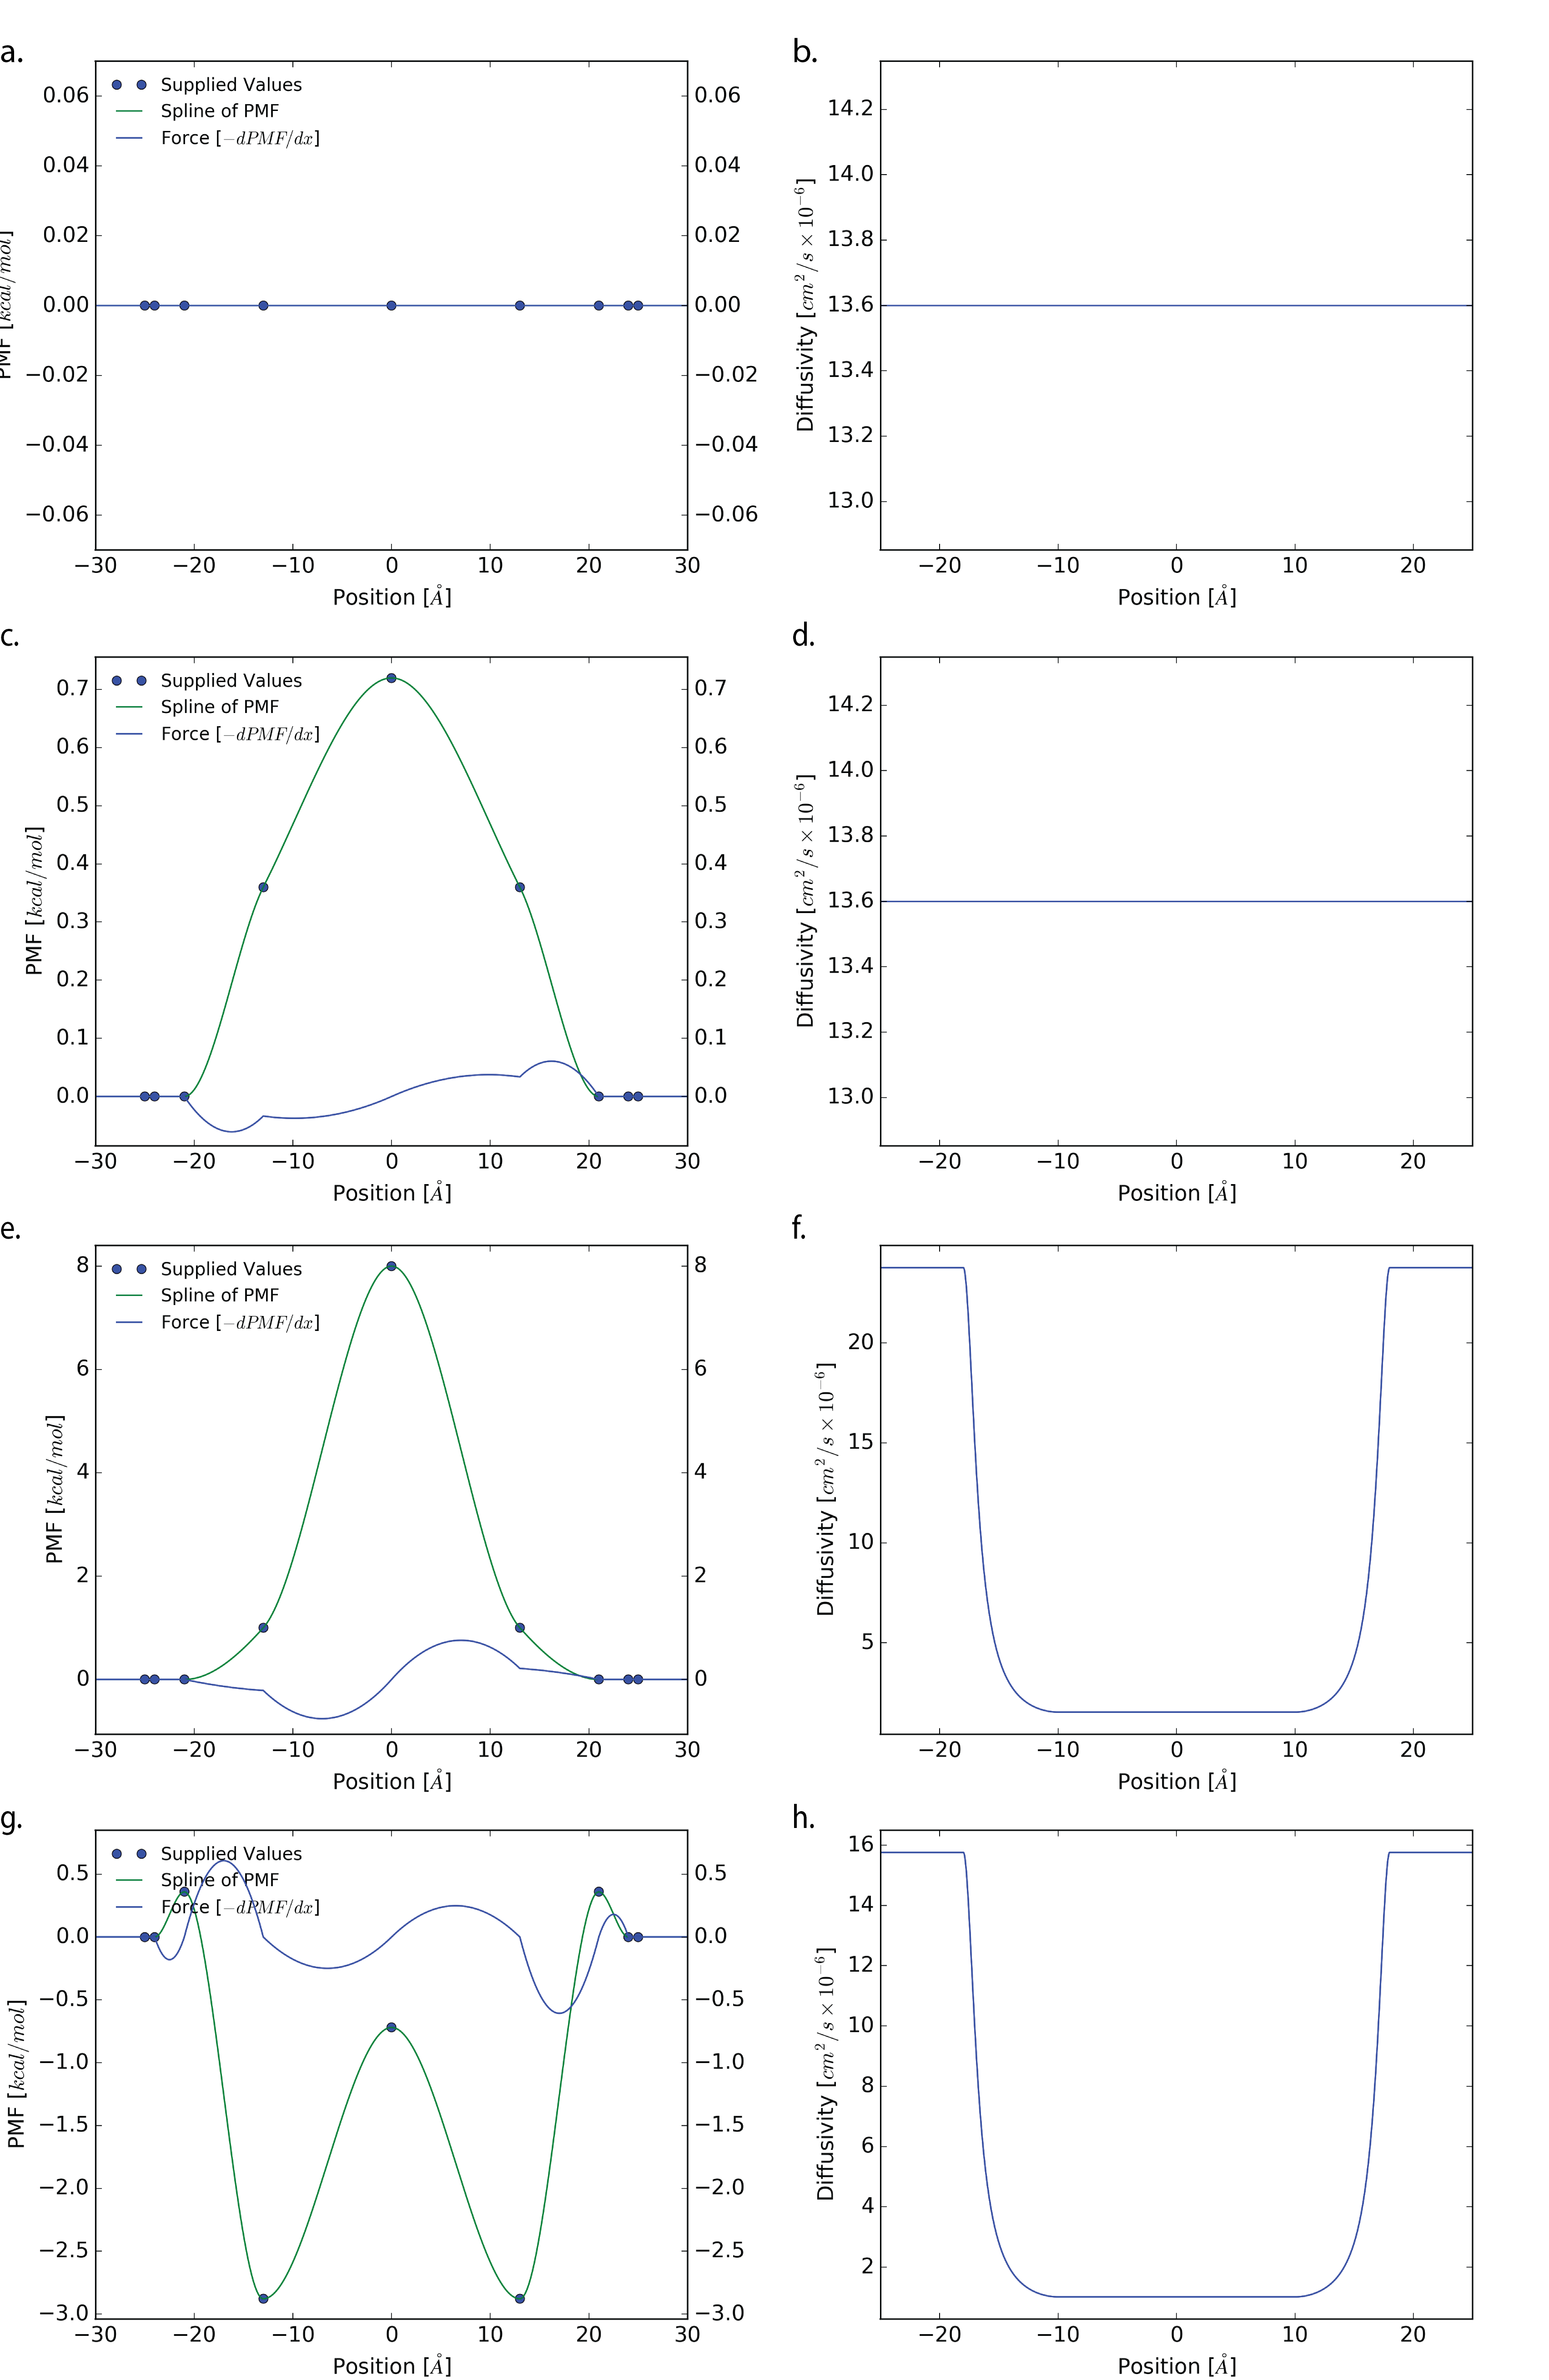
\includegraphics[width=0.8\textwidth]{Figures/profiles.png}
        \caption[PMF and diffusivity profiles assigned for toy systems]{The PMF and diffusivity profiles used for each system. Each profile is represented using a piecewise cubic Hermite polynomial interpolated from a set of user specified values.}
        \label{fig:profiles}
    \end{center}
    \end{figure}

    \par We integrate the Langevin equation using a velocity-Verlet-like integrator by Gr\o nbech-Jensen--Farago\cite{Gronbech-Jensen2013} to generate sample trajectories
    \begin{gather}
    q(t+dt) = q(t) + bdtv(t) + \frac{bdt^2}{2m}f(t) + \frac{bdt}{2m}\Gamma(t+dt),\\
    v(t+dt) = av(t) + \frac{dt}{2m}[af(t) + f(t+dt)] + \frac{b}{m}\Gamma(t+dt),\\
    b \equiv \frac{1}{1+\frac{cdt}{2m}},\\
    a \equiv \frac{1- \frac{cdt}{2m}}{1 + \frac{cdt}{2m}},
    \end{gather}
    where $q$ is the position, $t$ is the current time, $c$ the friction coefficient, $b$ and $a$ are unitless constants, $f$ is the force, $v$ the velocity, and $m$ the particle mass. This integrator was derived by integrating the noise term at a small time step $dt$. The new term, $\Gamma$, is Gaussian distributed and has the following properties:
    \begin{gather}
    \langle\Gamma(t+dt)\rangle = 0,\\
    \langle\Gamma(t)\Gamma(t')\rangle = 2ck_BTdt\delta(t,t').
    \end{gather}
    The quality of random number generators (RNG) to sample $\Gamma$ is shown in Fig.~S1. In this work, the aforementioned drag coefficient, $c$, is estimated by Stokes law,
    \begin{equation}
        F_d = \underbrace{6\pi\eta R_{hyd}}_{c}v,
    \end{equation}
    where $F_d$ is the frictional force. For additional information regarding the implementation details of the Langevin dynamics engine please refer to the SI.

    \begin{table}[ht]
    \centering
    \caption{Parameter inputs to the Langevin dynamics simulations for each case.}
    {
    \begin{tabular}{|c|c|c|c|c|}
        \hline
                            & Flat     & Small Barrier & Urea     & Codeine  \\\hline
        $R_{hyd}$ (\AA)     & 5        & 5             & 2.86     & 4.32     \\\hline
        Mass (g/mol)        & 20       & 20            & 60       & 299      \\\hline
        T (K)               & 298      & 298           & 298      & 298      \\\hline
        Brute dt (s)        & 1\e{-12} & 1\e{-12}      & 1\e{-12} & 1\e{-12} \\\hline
        Milestone dt (s)    & 1\e{-15} & 1\e{-15}      & 1\e{-15} & 1\e{-15} \\\hline
        \end{tabular}
    }
    \label{table:SimulationParameters}
    \end{table}

    \par Using the above dynamics engine, sample trajectories under various conditions can be generated. Here the permeability is calculated via several methods: 1) theoretical ISD, 2) theoretical MFPT-ISD, 3) brute forced MFPT-ISD, 4) milestoning MFPT-ISD, 5) brute PBCP, and 6) milestoning PBCP. Methods 1, 2 are directly evaluated numerically from the interpolated profiles using the relations in the Theory section. Methods 3--6 employ brute force or milestoning calculations to generate sample trajectories which are post-processed to yield the permeability coefficient. The strategy for brute force and milestoning simulations are described below.

    \subsection{Brute Force Sampling and Statistics}
        \par Brute force attempts to sample the membrane crossing event via a single continuous trajectory were attempted as follows: Trajectories to sample $\mfptm$  and $\rho$ were intiated at one end of the membrane $z=-25$~\AA, the \surf{a}. Trajectories to sample the MFPT employed reflecting boundary conditions at the start to prevent the particle from diffusing away into bulk. Effectively trajectories which passed the reflecting boundary at the \surf{a}, were place back across the boundary and velocity reversed. In contrast, the simulations to obtain $\rho$ have an absorbing boundary placed at $z=-26$~\AA, corresponding to the so-called \surf{q}. Trajectories that crossed the \surf{q} were halted and counted as non-crossing events.

        \par For all brute force trajectories, an absorbing boundary was placed at $z=25$~\AA. Upon crossing this terminal boundary, the simulations are halted and either the crossing time or the event recorded for the MFTP, and $\rho$ sampling cases respectively. The crossing probability was found according to
        \begin{equation}
            \rho = \frac{n_b}{n_b + n_q},
        \end{equation}
        where $n_b$ and $n_q$ are the number of $b-$ or \surf{q} crossing events observed. The FPT distribution often takes the form of a Poisson or exponential distribution. We attempt to quantify the quality of the MFPT estimate by computing the root mean square error (RMSE) of the population and confidence interval by bootstrapping. The RMSE is defined as
        \begin{equation}
            \sigma_{\mfptm} = \sqrt{\frac{1}{N}\sum_{i=1}^{N} (t_i - \mfptm)^2},
        \end{equation}
        where $t_i$ is the time that trajectory $i$ took before touching the absorbing boundary and $N$ is the total number of observations. We also report the 95\% confidence intervals of both the MFPT and the crossing probability. This is estimated by bootstrapping using the Bias-Corrected and Accelerated method and percentile method for the MFPT and crossing probabilities respectively with 10,000 resamples\cite{Efron1987,Efron1993}.

    \subsection{Milestoning}
        \par In this section we explain our experimental approach and include a brief description of milestoning theory. Milestones are spaced at $1$~\AA{} increments across the bilayer ($[-25,25]$), and in the case of $\rho$ estimation, an additional milestone was placed at $z = -26$~\AA. Trajectories were initiated with a position starting at each milestone, $M_i$, with a random velocity sampled from the Maxwell-Boltzmann distribution. Two stages are needed to obtain milestoning statistics. According to formal milestoning theory, we must determine the first hitting point distribution (FHPD) on $M_i$. To find the FHPD, trajectories are started at milestone $M_i$ and run until they cross either another milestone ($M_{i+1}$, $M_{i-1}$) or the originating milestone ($M_i$). If the trajectory is self-crossing then the simulation is halted and statistics discarded. Conversely, if the trajectory crosses an adjacent milestone first then this trajectory is a member of the FHPD on milestone $M_i$. Due to the microscopic time-reversiblity of classical mechanics, the reverse of this trajectory is a valid simulation of the crossing from ($M_{i+1},M_{i-1}\rightarrow M_{i}$). Thus we term this stage the ``reverse'' phase. Next we begin the ``forward'' phase where each member of the FHPD is restarted at $M_i$, but with the initial velocity vectors reversed. These trajectories propagate until they cross an adjacent milestone, $M_{i+1}$ or $M_{i-1}$. Self crossing events of the starting milestone $M_i$ are ignored in the forward phase.

        \par The forward phase provides all the transition and incubation time statistics that will be used in the milestoning analysis. As the milestones are crossed, each trajectory is counted, and the time that each trajectory took is also tracked. A transition kernel matrix $\mathbf{K}$ is then generated, whose elements $K_{ij}$ represent the transition probability that a system starting at milestone $M_i$ will transition to milestone $M_j$
        \begin{equation}
            K_{ij} = \frac {n_{i\rightarrow j}} {\sum_{k=1}^{N} n_{i \rightarrow k}},
        \end{equation}
        where $n_{i\rightarrow j}$ represents the total number of trajectories that cross from milestone $i$ to milestone $j$, where $N$ is the index of the final milestone. Similarly, a lifetime or incubation time vector $\boldsymbol{\tau}$ is also generated, whose elements $\tau_i$ represent the average time that a system spends in milestone $i$
        \begin{equation}
            \tau_{i} = \frac{\sum_{l=1}^{n_i} t_l} {n_i},
        \end{equation}
        where $t_l$ is the time that trajectory $l$ takes to reach an adjacent milestone, and $n_i$ is the total number of trajectories starting from milestone $i$.

        \par Using $\mathbf{K}$ and $\boldsymbol{\tau}$, we can compute thermodynamic quantities such as the stationary flux ($\mathbf{q_{stat}}$) and the stationary probability ($\mathbf{p_{stat}}$), as well as the MFPT (\mfpt), a kinetic quantity. First, we compute the stationary probability using the following eigenvalue equation
        \begin{equation}
            \mathbf{K} \mathbf{q_{stat}} = \mathbf{q_{stat}}.
            \label{eq:qstat}
        \end{equation}

        \par Note that before solving Eq.~\ref{eq:qstat}, we typically have to modify $\mathbf{K}$ to have the correct boundary conditions. For our membrane system, since the two terminal milestones at each end of the membrane have no additional milestones beyond them, it does not make sense to simulate from them. We can fill in reasonable transition probabilities and lifetimes using the following scheme: Since each terminal milestone only has one adjacent milestone, we can set the transition probability to transition to the singular neighbor or the other side of the membrane with equal probability. These are periodic boundary conditions. That is, for a set of milestones $\mathbf{M}={M_1, M_2, \ldots, M_N}$
        \begin{equation}
            K_{1i} =  \begin{cases}
                0.5 & \text{if } i=2 \\
                0.5 & \text{if } i=N \\
                0 & \text{if } i \neq 2,N
            \end{cases},
        \end{equation}
        and
        \begin{equation}
            K_{Ni} = \begin{cases}
                0.5 & \text{if } i = N-1\\
                0.5 & \text{if } i = 1\\
                0 & \text{if } i \neq 1,N-1
            \end{cases},
        \end{equation}
        where $N$ is the index of the last milestone and $i$ is a milestone index. Splitting the transition probabilities equally makes sense because these milestones are in the bulk solvent, where the PMF is flat. For the lagtime vector $\boldsymbol{\tau}$, given that the terminal milestones are in bulk solvent, the lagtime is defined as follows
        \begin{equation}
            \tau_0 = \tau_N = \frac{\Delta x^2}{2D},
        \end{equation}
        where $\Delta x$ is the cartesian distance to the adjacent milestone, and $D$ is the diffusivity coefficient in bulk. With these changes, we can estimate the stationary probability according to
        \begin{equation}
            p_{stat,i} = q_{stat,i} \cdot \tau_i,
        \end{equation}
        Where we take the element-wise product over all milestone indeces $i$.

        \par The stationary probability distribution, $\mathbf{p_{stat}}$, can be used to obtain an estimate of the underlying PMF, $W_i$, at milestone $i$ accordingly
        \begin{equation}
            W_i = -\beta^{-1}\log(p_{stat,i}/p_{stat,1}).
        \end{equation}
        We use this calculated PMF to estimate the integral in Eq.~\ref{eq:permmfpt} by performing a numerical integration.

        \par To find the MFPT needed to estimate the permeability in Eq.~\ref{eq:permmfpt}, we must modify the transition kernel $\mathbf{K}$ once again. This time, we must make milestone $M_N$ a ``draining'' state by setting all $K_{N, k} = 0$, $\forall k$. We also must modify transitions at milestone $M_1$ to transition only to its neighbor, milestone $M_2$:
        \begin{equation}
            K_{1i} = \begin{cases}
                1 & \text{if } i = 2\\
                0 & \text{if } i \neq 2
            \end{cases}.
        \end{equation}
        To get the MFPT, we then solve the following equation
        \begin{equation}
                \mfptm = \mathbf{p_0} \cdot (\mathbf{I}-\mathbf{K})^{-1} \cdot \boldsymbol{\tau},
        \end{equation}
        where $\mathbf{p_0}$ is a starting distribution of probabilities along the milestone. We choose $p_{0,i}$  to be 1 if $i = 1$, and choose $p_{0,i}$ to be 0 otherwise.

        \par Finally, we obtain the crossing probability $\rho$ for Eq.~\ref{eq:permrho} by further modifying the transition kernel $\mathbf{K}$. Recalling that the computation of $\rho$ requires an additional milestone at \surf{q}, which we assign index $i = 0$. We simulate starting from the other interior milestones. The first and last milestones become ``sink'' states that capture probability and never let it escape, thus; no simulations start from sink states, only end on them. Sink states are defined by setting
        \begin{equation}
            K_{0i} = \begin{cases}
                1 & \text{if } i = 1\\
                0 & \text{otherwise}
            \end{cases},
        \end{equation}
        and
        \begin{equation}
            K_{Ni} = \begin{cases}
                1 & \text{if } i = N\\
                0 & \text{otherwise}
            \end{cases}.
        \end{equation}
        Once again solving Eq.~\ref{eq:qstat} we obtain a stationary flux vector, $\mathbf{q_{stat}}$, which represents the proportion of systems that would have partitioned between the sink states at the ends of the membrane. The elements of the vector $\mathbf{q_{stat}}$, must be normalized such that all its elements sum to one for this calculation, however, since $\mathbf{K}$ is a Markov matrix, the eigenvector should already be normalized. Since milestone $M_N$ represents the \surf{a}, $\rho$ in Eq.~\ref{eq:permrho} can be extracted from the last value in $\mathbf{q_{stat}}$,
        \begin{equation}
            \rho = q_{stat,N}.
        \end{equation}

        \par The error is sampled according to the scheme found in Ref.~\citenum{Votapka2015}. For all milestoning values, we resample 1000 times and report the standard deviation of each measurable.

\section{Results and Discussion}
    \par Below we report the computed permeability coefficients and MFPTs according to the six methods: 1) the ISD, 2) ISD from MFPT, 3) ISD with brute forced MFPT, 4) milestoning estimated \mfpt in ISD, 5) brute force with no assumptions, and 6) milestoning with no assumptions in Table~\ref{table:milepermresults}. Note again that the brute forced MFPT is performed with a reflecting boundary condition at the starting position while no such condition is applied for the brute force crossing probabilities. This explains the reported brute force MFPT without any crossings observed for the urea system.


\begin{table}[htbp]
\small
\centering
\caption{The computed MFPT and permeability coefficients according to each method. Reported error bars for the MFPT corresponds to the RMSE while the error for the crossing probability is from bootstrapping. Error in the brute force log permeability is estimated by the mean log($P$) difference of the high and low confidence intervals. $^{\dagger}$ We observed no brute force crossing transitions for the urea system. The values in parentheses represent the number of forward-phase trajectories sampled in each case.}
\begin{sideways}
\begin{tabular}{|c|p{2.25cm}|p{2.25cm}|p{2.25cm}|p{2.25cm}|}
    \hline
                            & Flat                          & Small Barrier
                                    & Urea                           & Codeine                   \\\hline
    Theoretical MFPT (s)    & 9.19\e{-9}                    & 1.11\e{-8}
                                    & 1.99\e{-3}                     & 2.89\e{-7}                \\\hline

    Brute Forced MFPT (s)   & 9. $\pm$ 7. \e{-9} (5100)     & 1.1 $\pm$ 1.0\e{-8} (2500)
                                    & 3. $\pm$ 3.\e{-4} (1694)       & 10. $\pm$ 9.\e{-7} (1600) \\\hline

    Milestoning MFPT (s)    & 1.15 $\pm$ 0.05\e{-8}         & 1.35 $\pm$ 0.04\e{-8}
                                    & 1.9 $\pm$ 0.3\e{-3}        & 4.0 $\pm$ 0.3\e{-7}        \\\hline\hline

    \textbf{Crossing Probability} ($\boldsymbol{\rho})$ & & & & \\\hline
    Brute Force             & 2.7 $\pm$ 0.8\e{-2} (1722)    & 1.0 $\pm$ 0.4\e{-2} (2500)
                                    & --$^{\dagger}$ (1627)          & 7. $\pm$ 1.\e{-2} (1340)  \\\hline

    Milestoning             & 1.7 $\pm$ 0.1\e{-2}           & 9.8 $\pm$ 0.5\e{-3}
                                    & 3.1 $\pm$ 0.4\e{-8}            & 2.2 $\pm$ 0.3\e{-2}     \\\hline\hline

    \textbf{Permeability log(cm/s)} & & & & \\\hline
    1) ISD                  & 1.43            & 1.14             & -4.33            & 1.44           \\\hline
    2) MFPT-ISD             & 1.43            & 1.14             & -4.33            & 1.44           \\\hline
    3) Brute Force MFPT-ISD & 1.43 $\pm$ 0.01 & 1.14 $\pm$ 0.01  & -3.49 $\pm$ 0.02 & 0.91 $\pm$ 0.02\\\hline
    4) Milestoning MFPT-ISD & 1.33 $\pm$ 0.03 & 1.06 $\pm$ 0.02  & -4.3 $\pm$ 0.09  & 1.35 $\pm$ 0.06\\\hline
    5) Brute Force PBCP     & 1.6 $\pm$ 0.1   & 1.1 $\pm$ 0.2    & --               & 2.04 $\pm$ 0.09\\\hline
    6) Milestoning PBCP     & 1.37 $\pm$ 0.03 & 1.13 $\pm$ 0.02  & -4.13 $\pm$ 0.06 & 1.54 $\pm$ 0.04\\\hline
    \end{tabular}
\end{sideways}
\label{table:milepermresults}
\end{table}

    \par The distribution of the mean first passage times is shown in Fig.~\ref{fig:mfpts}. Due to the highly tailed nature of the MFPT, it is difficult to estimate it from brute force simulations. Milestoning greatly aids in the computation of the first passage times by reducing the total distance between points of interest. Using clever statistics, milestoning theory is capable of reconstructing the MFPT from many short simulations. For all cases, we obtain MFPTs in good agreement with the theoretical results. Deviations in both the brute force and milestoning cases are likely caused by insufficient sampling. Sampling convergence for the milestoning can be visualized by deviations in the milestoning-derived PMF from the actual PMF.

    \begin{figure}[htbp]
    \begin{center}
        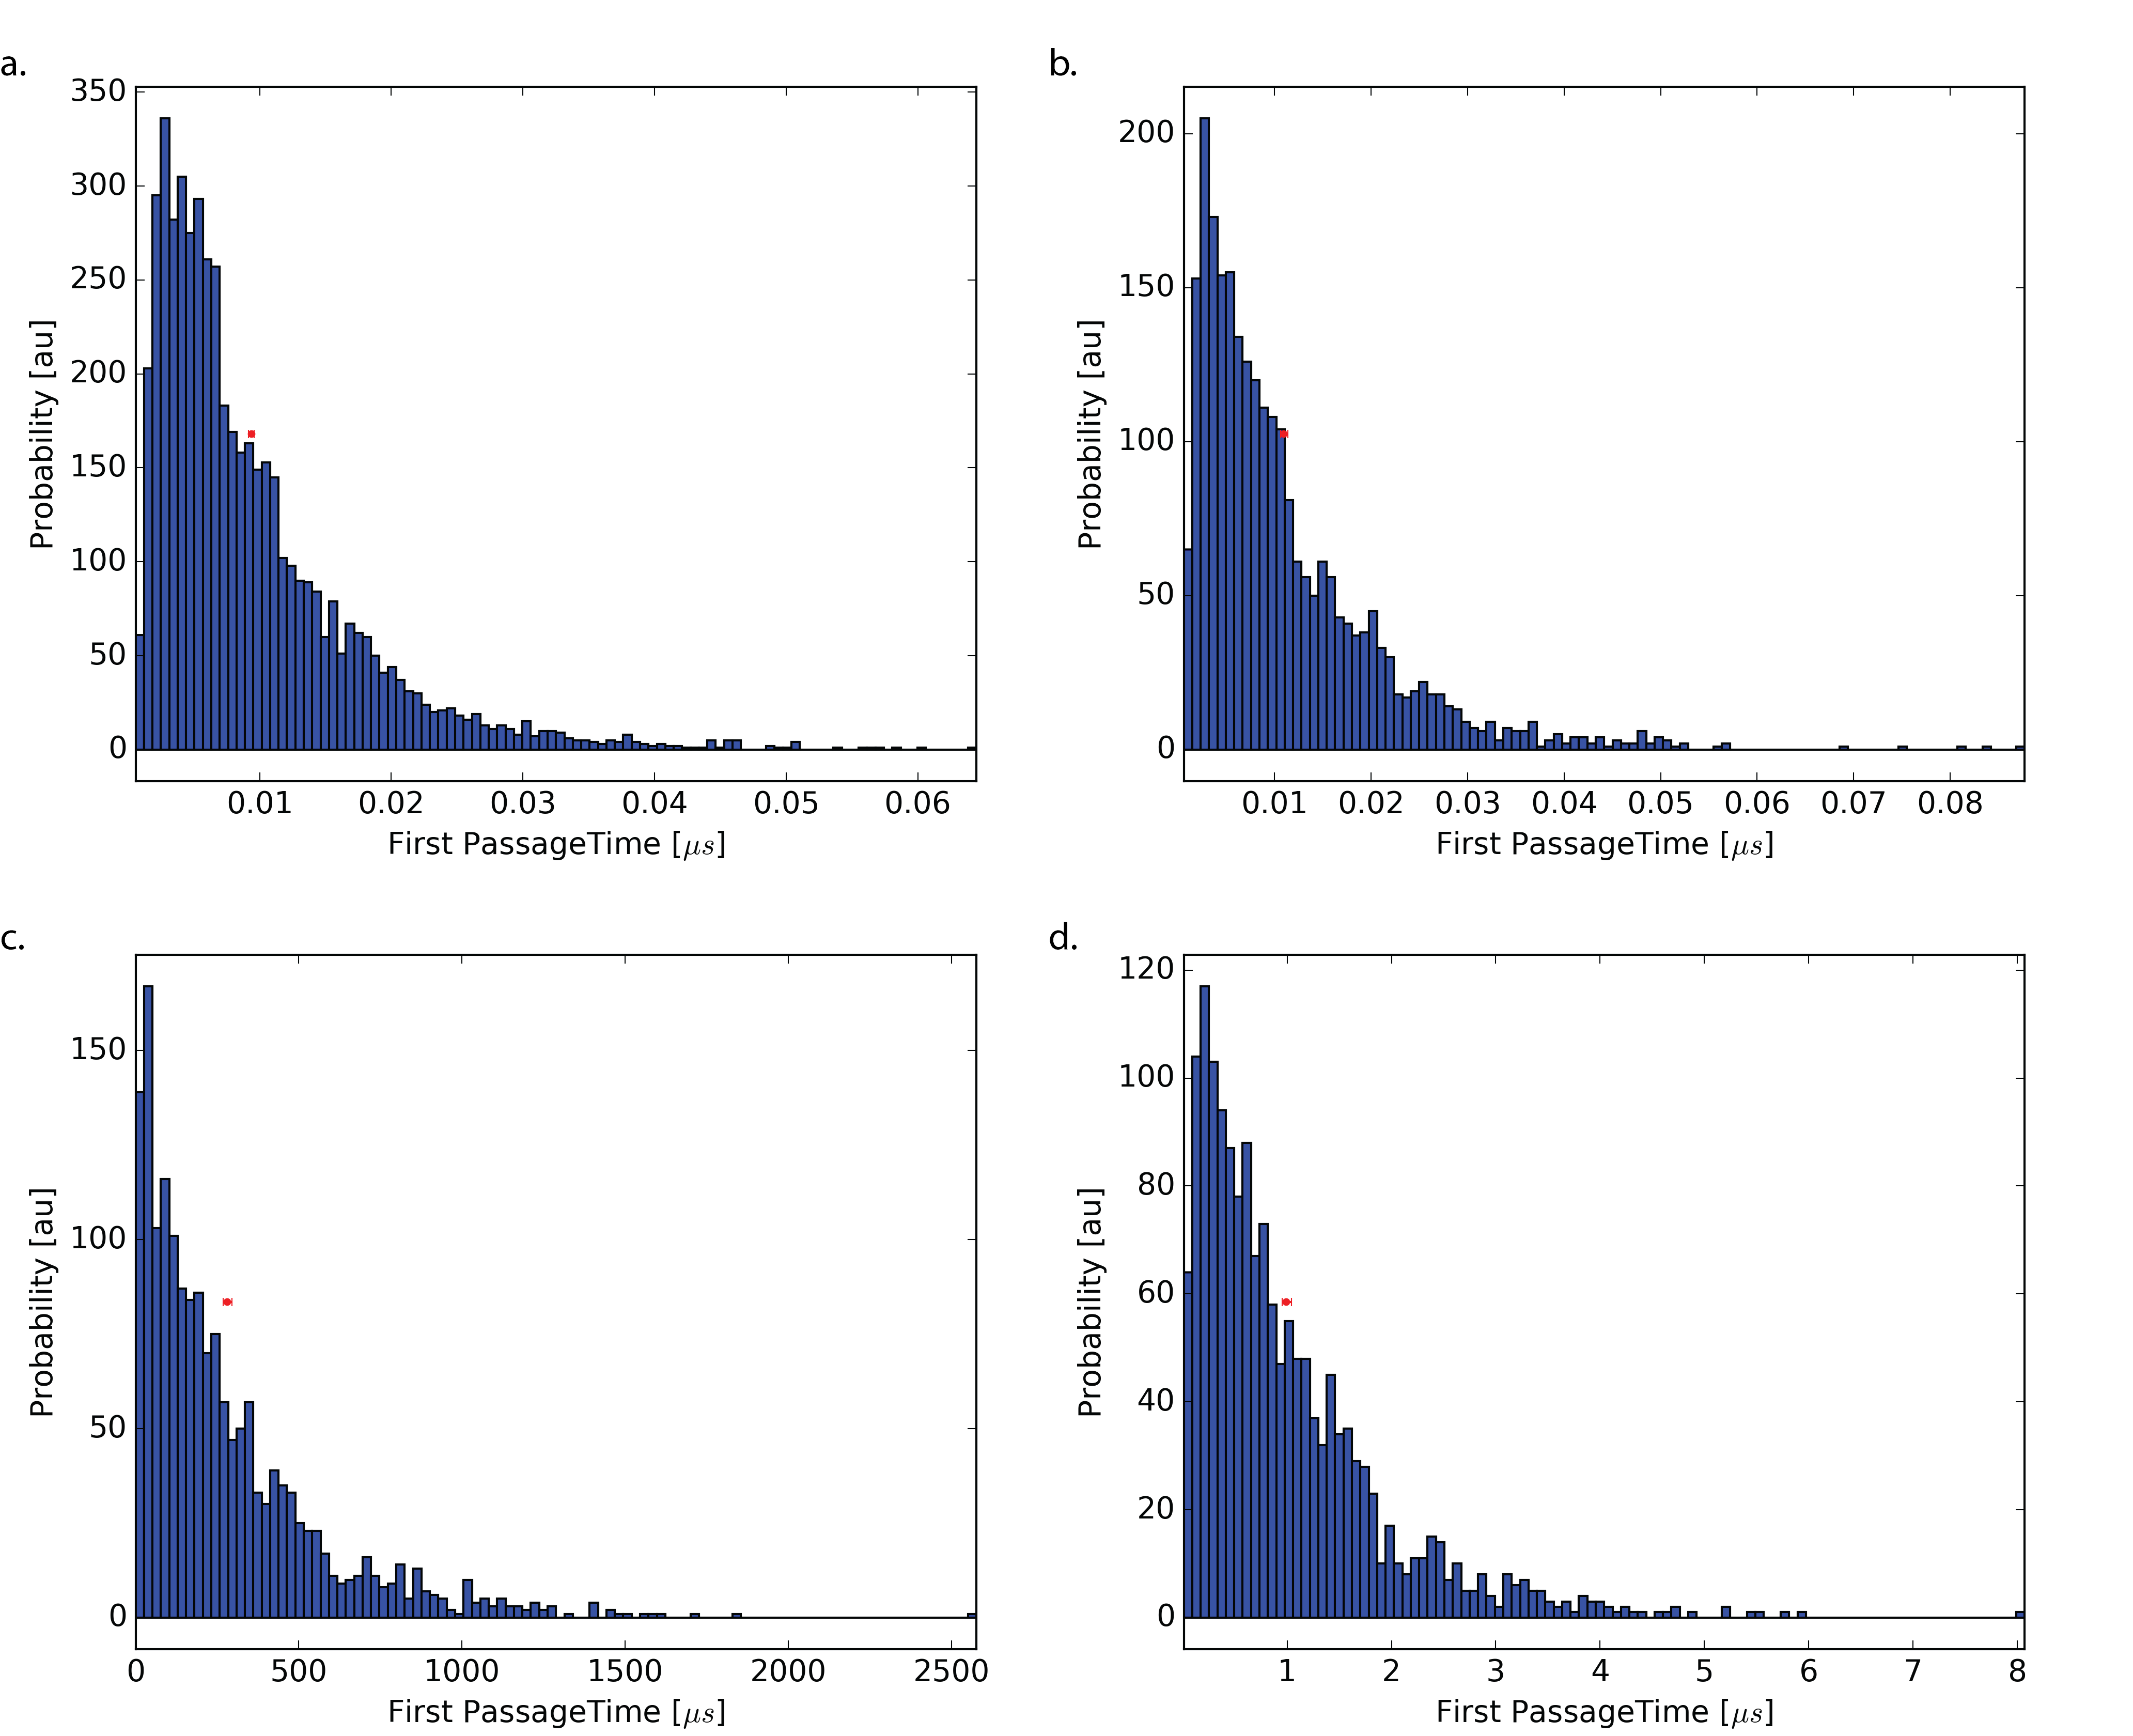
\includegraphics[width=0.8\textwidth]{Figures/mfptdist}
        \caption[Distributions of brute force MFPTS for systems (a) flat, (b) small-barrier, (c) urea, and (d) codeine]{Shown here are the distributions of the brute force MFPTs for systems (a) flat, (b) small-barrier, (c) urea, and (d) codeine. Due the presence of large barriers in the urea and codeine cases, the sampling is limited. The red points and error bars indicate the mean and boostrapped 95\% confidence intervals of the MFPT.}
        \label{fig:mfpts}
    \end{center}
    \end{figure}

    \par Reconstructed PMF profiles from milestoning are shown in Fig.~\ref{fig:calcpmf}. Here we see that the estimated potentials of mean force are relatively converged. Discrepancies are more prevalent along $-18<z<18$ where the membrane exists. We suspect that the increased viscosity leads to additional self-crossing events during the reverse phase thus hindering the overall sampling. The total amount of collected statistics per milestone for each system is shown in Fig.~S2. With milestoning, we can easily adaptively sample regions of poor convergence.

    \begin{figure}[htbp]
    \begin{center}
        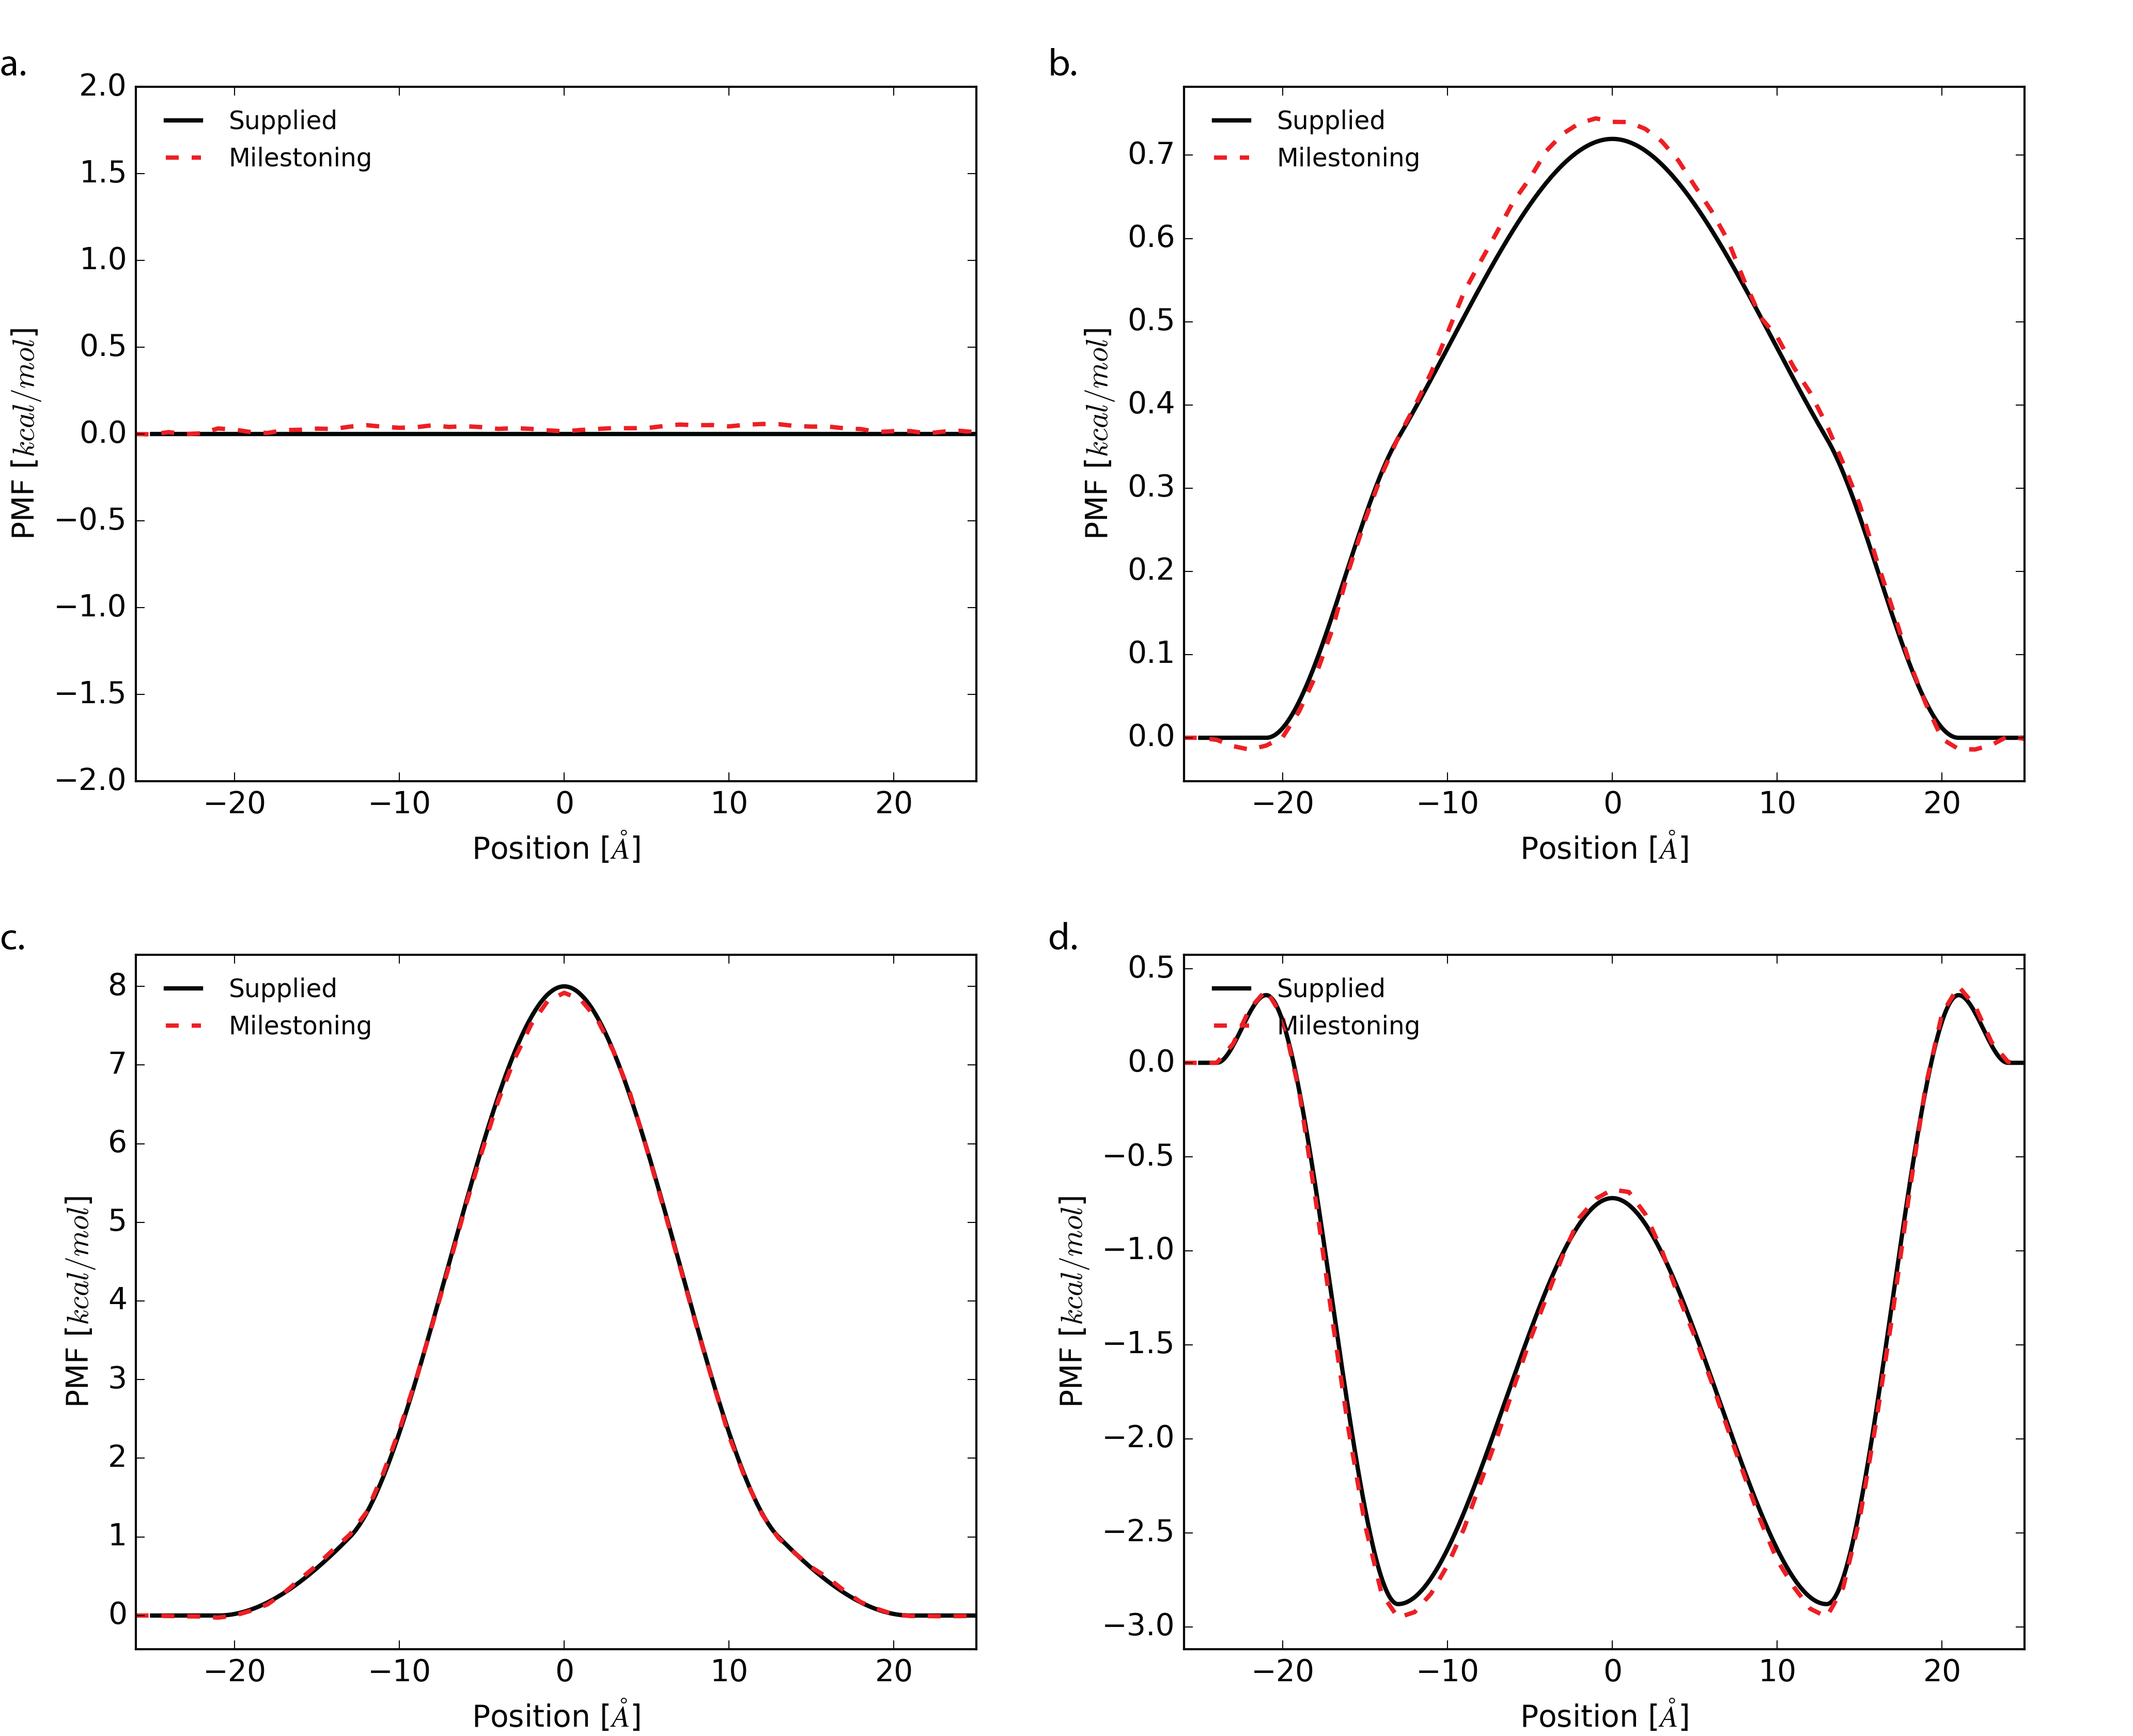
\includegraphics[width=0.8\textwidth]{Figures/calcpmf}
        \caption[PMF profiles of each system (a) flat, (b) small-barrier, (c) urea, and (d) codeine]{PMF profiles of each system: (a) flat, (b) small-barrier, (c) urea, and (d) codeine as estimated by milestoning, dotted red. The actual PMF is shown in black.}
        \label{fig:calcpmf}
    \end{center}
    \end{figure}

	\par By comparing and utilizing the two equations derived, Eq.~\ref{eq:permmfpt} and Eq.~\ref{eq:permrho}, the difference in the derivations must be considered for proper analysis and application. Eq.~\ref{eq:permmfpt} was derived using the Smoluchowski equation, which assumes that the underlying system dynamics is overdamped. This assumption is also used in the widely employed ISD, Eq.~\ref{eq:ihsd}. Our relation of the MFPT to the permeability does not require the estimation of a position dependent diffusion tensor. While there are many methods for calculation of the local diffusivity, these methods suffer largely from convergence issues\cite{Mamonov2006,Lee2016}. The theory of milestoning does not compute diffusion coefficient directly, but rather estimates rates of passage, probability, and flux. Using Eq.~\ref{eq:permmfpt}, the MFPT from milestoning can be used to compute permeability coefficients along with the stationary probability. To the best of our knowledge, this formulation of the ISD using the MFPT has not been shown previously.

	\par As aforementioned, the assumption that the dynamics inside of the bilayer are over-damped is largely untested. Several instances of anomalous diffusion have been observed in crowded environments among many others\cite{Sokolov2012,Banks2005,Regner2013,Berezhkovskii2014a,McGuffee2010}. Similarly, the dynamics of water near hydrophobic surfaces is often complicated\cite{Setny2013}. Thus we present a formula relating the permeability to the crossing  probabilities, $\rho$, which makes no assumptions about the dampedness. While the Smoluchowski equation is used in the derivation of Eq.~\ref{eq:permrho}, it was only used in the regions containing bulk solvent. Remaining transport properties are encapsulated by the probability $\rho$, which, when calculated from milestoning, makes no assumptions about the dynamics.

	\par Our scheme is similar to that proposed by Cardenas et. al.\cite{Cardenas2013,Cardenas2014} excepting that we obviate the need to compute the stationary flux across the first milestone by Langevin dynamics simulations. In Eq.~\ref{eq:permrho}, the flux across the first milestone is captured by our system of two Smoluchowski equations. Therefore, we eliminate a potentially cumbersome, albeit inexpensive, step in the estimation of the permeability coefficient.

	\par We also demonstrated the utility and accuracy of both of the derived equations using a 1-D Langevin dynamics model with various  PMF and diffusion profiles. In the case of the flat profile, the results of the simulations, both brute-force and milestoning, can be directly compared with theoretically derived results. For all cases, the theoretical ISD and MFPT-ISD were the same. This is not suprising, given that both are derived from equivalent expressions. Comparing the brute forced MFPT-ISD to the theoretical for the flat profile, we see that they are also comparable within error. In contrast, the flat milestoning PBCP yields a permeability coefficient that was smaller than predicted by the ISD. This discrepancy could be an example of how dampedness plays a role in the difference between the true and predicted permeability coefficients. Since the molecule simulated was not perfectly overdamped, there may be artifacts from conservation of momentum in Langevin dynamics, the formula using $\rho$ may have captured the influence of that effect.  Considering that an overdamped integrator would likely have yielded permeabilities that were more consistent between the two equations, one may question why we used the more general Langevin integrator in our test simulations. While an overdamped simulation integrator would have allowed us to apply Eq. 21 more accurately, we wanted to closely reproduce the situation that would be encountered in practical application of these equations, for instance, during an all-atom MD simulation with milestones across a bilayer, where an assumption of overdamped diffusion would not necessarily hold. For this reason, we also wanted to observe how different the predicted permeabilities would be for the same trajectories using the two different formulas.
	We anticipate that additional investigations of various permeabilities using all-atom molecular dynamics with milestoning may yield helpful insight about the structural characteristics of the bilayer by comparing the permeabilities estimated using Eqs. 21, 30.

	\par The two drug-like molecules that we simulated, urea and codeine, provide insight about the potential usefulness of using milestoning to approach practical permeability problems. We obtain quantitatively accurate results for both urea and codeine. Unfortunately, no crossing events for urea were observed by brute force despite substantial efforts. The effect of increased sampling on transition probabilities is explored using bootstrapping in Fig.~S3. Due to the presence of large transition barriers, the brute force calculation of permeability is intractable, excepting potentially the use of hyperspecialized hardware such as Anton\cite{Shaw2008}. Milestoning theory provides a framework for the estimation of membrane permeability using the MFPT in combination with transition probabilities via either the MFPT-ISD or the PBCP.

\section{Conclusions}
    \par We have derived two useful new relations for the calculation of permeability: first, a relation of the ISD to the MFPT assuming over-damped dynamics; second, we derive the PBCP which is agnostic to the underlying diffusional dynamics. Using simulations of our toy systems, we have demonstrated the utility and validity of each method. By comparing results obtained by the two methods, one can gain insight into the deviations of the permeability coefficient when the over-damped assumption is not valid. We anticipate that both approaches will be useful to the computational biophysical community when estimating permeability coefficients across membranes, particularly in the case when milestoning is being used in combination with molecular simulation to determine permeabilities.

    \section{Acknowledgements}
        \par \cref{chap:mileperm} is a modified reprint of the material as it appears in ``Votapka, L. W.; Lee, C. T.; Amaro, R. E. Two Relations to Estimate Membrane Permeability Using Milestoning. J. Phys. Chem. B 2016, 120 (33), 8606–8616. https://doi.org/10.1021/acs.jpcb.6b02814.''
        The dissertation author was the co-primary investigator and author of this paper.

        \par LWV acknowledges support from the National Science Foundation Graduate Research Fellowship Program (DGE-1144086). CTL acknowledges support from the NIH Molecular Biophysics Training Program (T32-GM008326). REA acknowledges a NIH Directors New Innovator Award DP2 OD007237, the National Biomedical Computation Resource (NBCR) NIH P41 GM103426, and supercomputing resources provided by XSEDE (NSF TG-CHE060073). REA is a co-founder of Actavalon, Inc. We also thank Gary Huber for the correction in the permeability of Eq.~\ref{eq:permrho} due to the resistivity of the bulk water. We would like to thank Rob Swift for insightful discussions on statistics and permeation physics. We also thank Professor Andy McCammon for his tireless mentorship, his impeccable theoretical and computational contributions, and for his unsurpassed vision in leading the field for all these years.
